\subsection{Steering generation to a region of PCA space}\label{sec:cond}
A PCA coordinate of a one-hot sequence is a projection, and since each site carries a single $1$
it is a sum of one table entry per site, $\mathrm{PC}_c(\bm x)=\sum_iV_c(i,x_i)-m_c$. The square of
such a sum contains only site and pair terms, so a harmonic restraint towards a target $\bm t$,
\begin{equation}
E_\lambda(\bm x)=E(\bm x)+\tfrac{\lambda}{2}\textstyle\sum_c\big(\mathrm{PC}_c(\bm x)-t_c\big)^2 ,
\label{eq:restraint}
\end{equation}
is itself a Potts energy, with couplings $\Delta J_{ij}(a,b)=-\lambda\sum_cV_c(i,a)V_c(j,b)$ and a field
linear in $\bm t$. Its Boltzmann distribution is the model's $p(\bm x)$ times a Gaussian window of
width $1/\sqrt\lambda$ around $\bm t$: the posterior given a noisy measurement of the coordinate.
We compare two ways of using it. \textbf{C1} adds Eq.~\eqref{eq:restraint} to the trained model at
sampling time, with no retraining. \textbf{C3} learns the conditional: per-site fields that depend
on the coordinates through $\phi(\bm z)=(1,u_1,u_2,u_1^2,u_2^2,u_1u_2)$ are trained with the couplings
on pairs $(\bm x,\mathrm{PC}(\bm x)+\sigma\bm\epsilon)$ and sampled at $\bm z=\bm t$; with blurred
coordinates it is fitted to the same distribution as C1 at $\lambda=1/\sigma^2$. A gain $\kappa$ on
its $\bm z$-dependent field mimics the coupling amplification $\beta_\mathrm{PCA}$ of an earlier
approach that appended discretised coordinates to the sequence as extra sites.

Targets are the three cluster centres of Sec.~\ref{sec:missing}; $3000$ chains per setting start
from random training sequences and run $500$ sweeps, and every pool is scored at that size against
the natural test sequences of the target cluster (Table~\ref{tab:cond}). Both methods use a
field-free model trained with longer patience (best epoch \EpBase\ rather than \EpClean). Its
validation pseudo-likelihood is $0.2$ nats better, yet it samples the clusters in proportions
\ShareBasep\ instead of \ShareClean\ (natural \ShareNat): the balance between the two major
clusters moved by $2.7$ nats of free energy, while \MissCl\ stayed at $5\%$. Pseudo-likelihood pins
down the conditionals, not the weights of the basins.

\begin{table*}[t]\centering\small\setlength{\tabcolsep}{4pt}
\begin{tabular}{lccccc}
\toprule
 & in target (\%) & distance & $r(C_{ij})$ & HPD (\%) & diversity \\
\midrule
unconditional baseline & 5/86/10 & 3.9/1.5/3.3 & 0.16/0.42/0.34 & 99/99/99 & 0.62/0.62/0.62 \\
rejection from baseline & 100/100/100 & 1.8/1.2/1.2 & 0.25/0.50/0.49 & 97/99/98 & 0.69/0.59/0.68 \\
\midrule
C1 $\lambda{=}1$ & 80/100/88 & 1.6/0.9/1.0 & 0.44/0.47/0.57 & 96/99/98 & 0.70/0.56/0.65 \\
C1 $\lambda{=}4$ & 100/100/100 & 0.6/0.5/0.5 & 0.46/0.39/0.60 & 96/99/99 & 0.64/0.52/0.62 \\
C1 $\lambda{=}16$ & 100/100/100 & 0.3/0.3/0.3 & 0.37/0.30/0.54 & 96/99/98 & 0.61/0.48/0.61 \\
\midrule
C3 $\sigma{=}1$ & 100/100/100 & 0.7/0.9/0.7 & 0.47/0.48/0.64 & 100/99/99 & 0.63/0.56/0.62 \\
C3 $\sigma{=}0.5$ & 100/100/100 & 0.4/0.5/0.5 & 0.38/0.40/0.60 & 100/100/100 & 0.57/0.52/0.61 \\
C3 $\sigma{=}0.25$ & 100/100/100 & 0.3/0.3/0.4 & 0.33/0.34/0.56 & 100/99/99 & 0.56/0.48/0.60 \\
\midrule
C3 $\sigma{=}0.5$, $\kappa{=}4$ & 100/100/100 & 1.5/0.9/1.8 & 0.12/0.18/0.29 & 100/100/92 & 0.29/0.31/0.55 \\
C3 $\sigma{=}0.5$, $\kappa{=}8$ & 100/100/100 & 1.6/1.2/1.8 & 0.08/0.08/0.12 & 100/100/56 & 0.16/0.21/0.40 \\
\midrule
natural (ceiling) & 100/100/100 & 1.0/1.3/0.8 & 0.66/0.63/0.75 & 100/100/99 & 0.67/0.60/0.64 \\
\bottomrule
\end{tabular}

\caption{Conditioning on each of the three cluster centres; every entry lists C0/C1/C2. In target:
fraction of samples landing in the target cluster. Distance: mean $\|\mathrm{PC}-\bm t\|$.
$r(C_{ij})$: against the natural test sequences of that cluster. HPD: fraction retaining the
J-domain motif. Diversity: mean pairwise Hamming distance inside the pool. Rejection keeps the
unconditional samples that fall in the cluster ($496$, $3000$, $948$ of $10^4$). Ceiling: $3000$
natural training sequences of the cluster.}
\label{tab:cond}
\end{table*}

\begin{figure*}[t]\centering
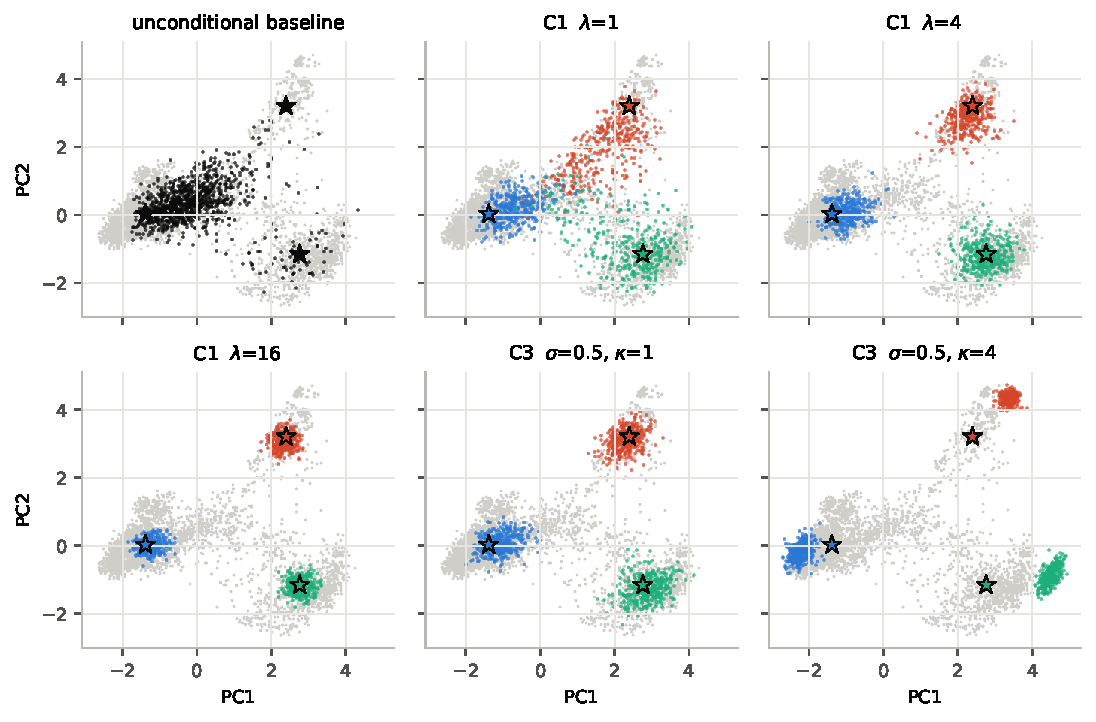
\includegraphics[width=0.84\textwidth]{../outputs/figures/cond_pca.pdf}
\caption{Conditioned samples in the PCA plane (grey: natural test). Stars: targets; points are
coloured by the target they were aimed at. Top left: unconditional sampling, which visits C1 almost
exclusively. Bottom right: C3 with its target field amplified ($\kappa=4$) --- every pool overshoots.}
\label{fig:condpca}
\end{figure*}

\textbf{C1 reaches every target and keeps the protein.} Without the restraint $5\%$ of the chains
end in \MissCl; from $\lambda=4$ on, all of them do (Fig.~\ref{fig:condpca}). The distance to the
target falls as $1/\sqrt\lambda$ --- the width of the window --- and responds monotonically to
$\lambda$, in contrast to the earlier $\beta_\mathrm{PCA}$. The HPD motif survives in $96$--$99\%$ of
samples at every stiffness. Agreement with the cluster's covariation peaks at
$\lambda\approx1$--$4$ ($r(C_{ij})=\ConeALfourrC$ for C0 and $0.60$ for C2, ceilings \CeilA\ and
\CeilC) and falls for stiffer restraints, mostly because a window much narrower than a natural
cluster samples its centre rather than the cluster. C1 is also far cheaper than rejection sampling,
which needs $10^4$ unconditional samples to yield $496$ in \MissCl, and it agrees with it: both give
C0 sequences of energy ${\approx}-106$, i.e.\ $14$ units above natural C0 (\NatEA). C1 samples the
model's own conditional, so it reaches the neglected region but inherits the model's view of it.

\textbf{C3 matches C1, and does better where the model is wrong.} At $\kappa=1$, C3 lands on target
with the accuracy and quality of C1 at the matching $\lambda=1/\sigma^2$, as the equivalence above
predicts. The exception is \MissCl: C3 reaches it at weak conditioning where C1 stops short
(distance $0.74$ vs $1.59$) and its C0 samples have lower energy (\CthreeAsHKoneE\ vs
\ConeALfourE), closer to natural. C1 reweights the unconditional model and carries its free-energy
error; C3 learned the conditional from data and does not.

\textbf{Amplifying the conditioning field reproduces the earlier failure.} At $\kappa=2,4,8$ the
samples overshoot by up to $1.5$ PC units, diversity collapses towards copies of one sequence
($0.16$ at $\kappa=8$), $r(C_{ij})$ falls to ${\sim}0.1$ and C2 loses the HPD motif in $44\%$ of
samples. Expanding Eq.~\eqref{eq:restraint} explains it: the exact conditional pairs a field pushing
towards $\bm t$ with a coupling term holding the coordinate \emph{at} $\bm t$, and $\kappa$ --- like
$\beta_\mathrm{PCA}$ --- amplifies the push without the spring.
